\chapter{Introduction}

In the quiet observation of the reality surrounding us, the attention of the human eye is often captured by the recognition of patterns, some structures, regularities or even symmetries repeating themselves across space and time. In Physics, symmetries are not only just an esthetical feature of Nature but is more of a guiding principle that underlies the formulation of physics laws. Over time, the study of such symmetries have shaped the way physicist have described the fundamental interaction governing the Universe. One of the multiple consequences of this perspective is known as Emmy Noether's first theorem she enunciated in 1915. In its general form, the theorem states that: 
\begin{center}
  \textit{'To every differentiable symmetry generated by local actions, there corresponds a conserved current'}
\end{center}

This statement is deeply connected to a more fundamental principle and requirement for any physical law: covariance. Noether's theorem provides a mathematical framework for expressing conservation laws through continuity equations. Initially applied to the explanation of conservation of energy, momentum and angular momentum through the symmetries of space and time in classical physics, it is now a pillar of modern theoretical physics, influencing fields such as Quantum Field Theory or General Relativity. \\
As of now, the description of the fundamental constituents of matter is performed by the Standard Model of particle physics, based itself on the rigorous mathematical framework of Quantum Field Theory. 
The Standard Model was developed in the early 1970s and is yet the best description of the fundamental constituents of matter, the particles, and the fundamental forces governing them. It has not only allowed physicist to perform precise predictions on a wide variety of phenomena but also to give explanation to almost all the experimental results obtained until now. \\ 

The matter particles all share one property which is their spin of one-half, they are hence called fermions. These later can further be divided into two subgroups, the quarks and the leptons, themselves divided into three generations depending on their stability. The first generation is associated with the lighter and thus more stable particles while the two other generations are associated to heavier and thus less stable particles. For this reason, the particles of the first generation are the ones we identify as components of the stable matter observed in the Universe.
There are four know fundamental forces acting on the particles, but only three of them are described by the Standard Model, the outlier being the gravitational force. Each of the forces is associated to the exchange of force-carriers particles which all have an integer value for their spin, they are hence called bosons. One last boson completes the model, the Higgs boson, responsible for the mass of the particles. \\ \clearpage

\begin{figure}[h]
	\centering
 	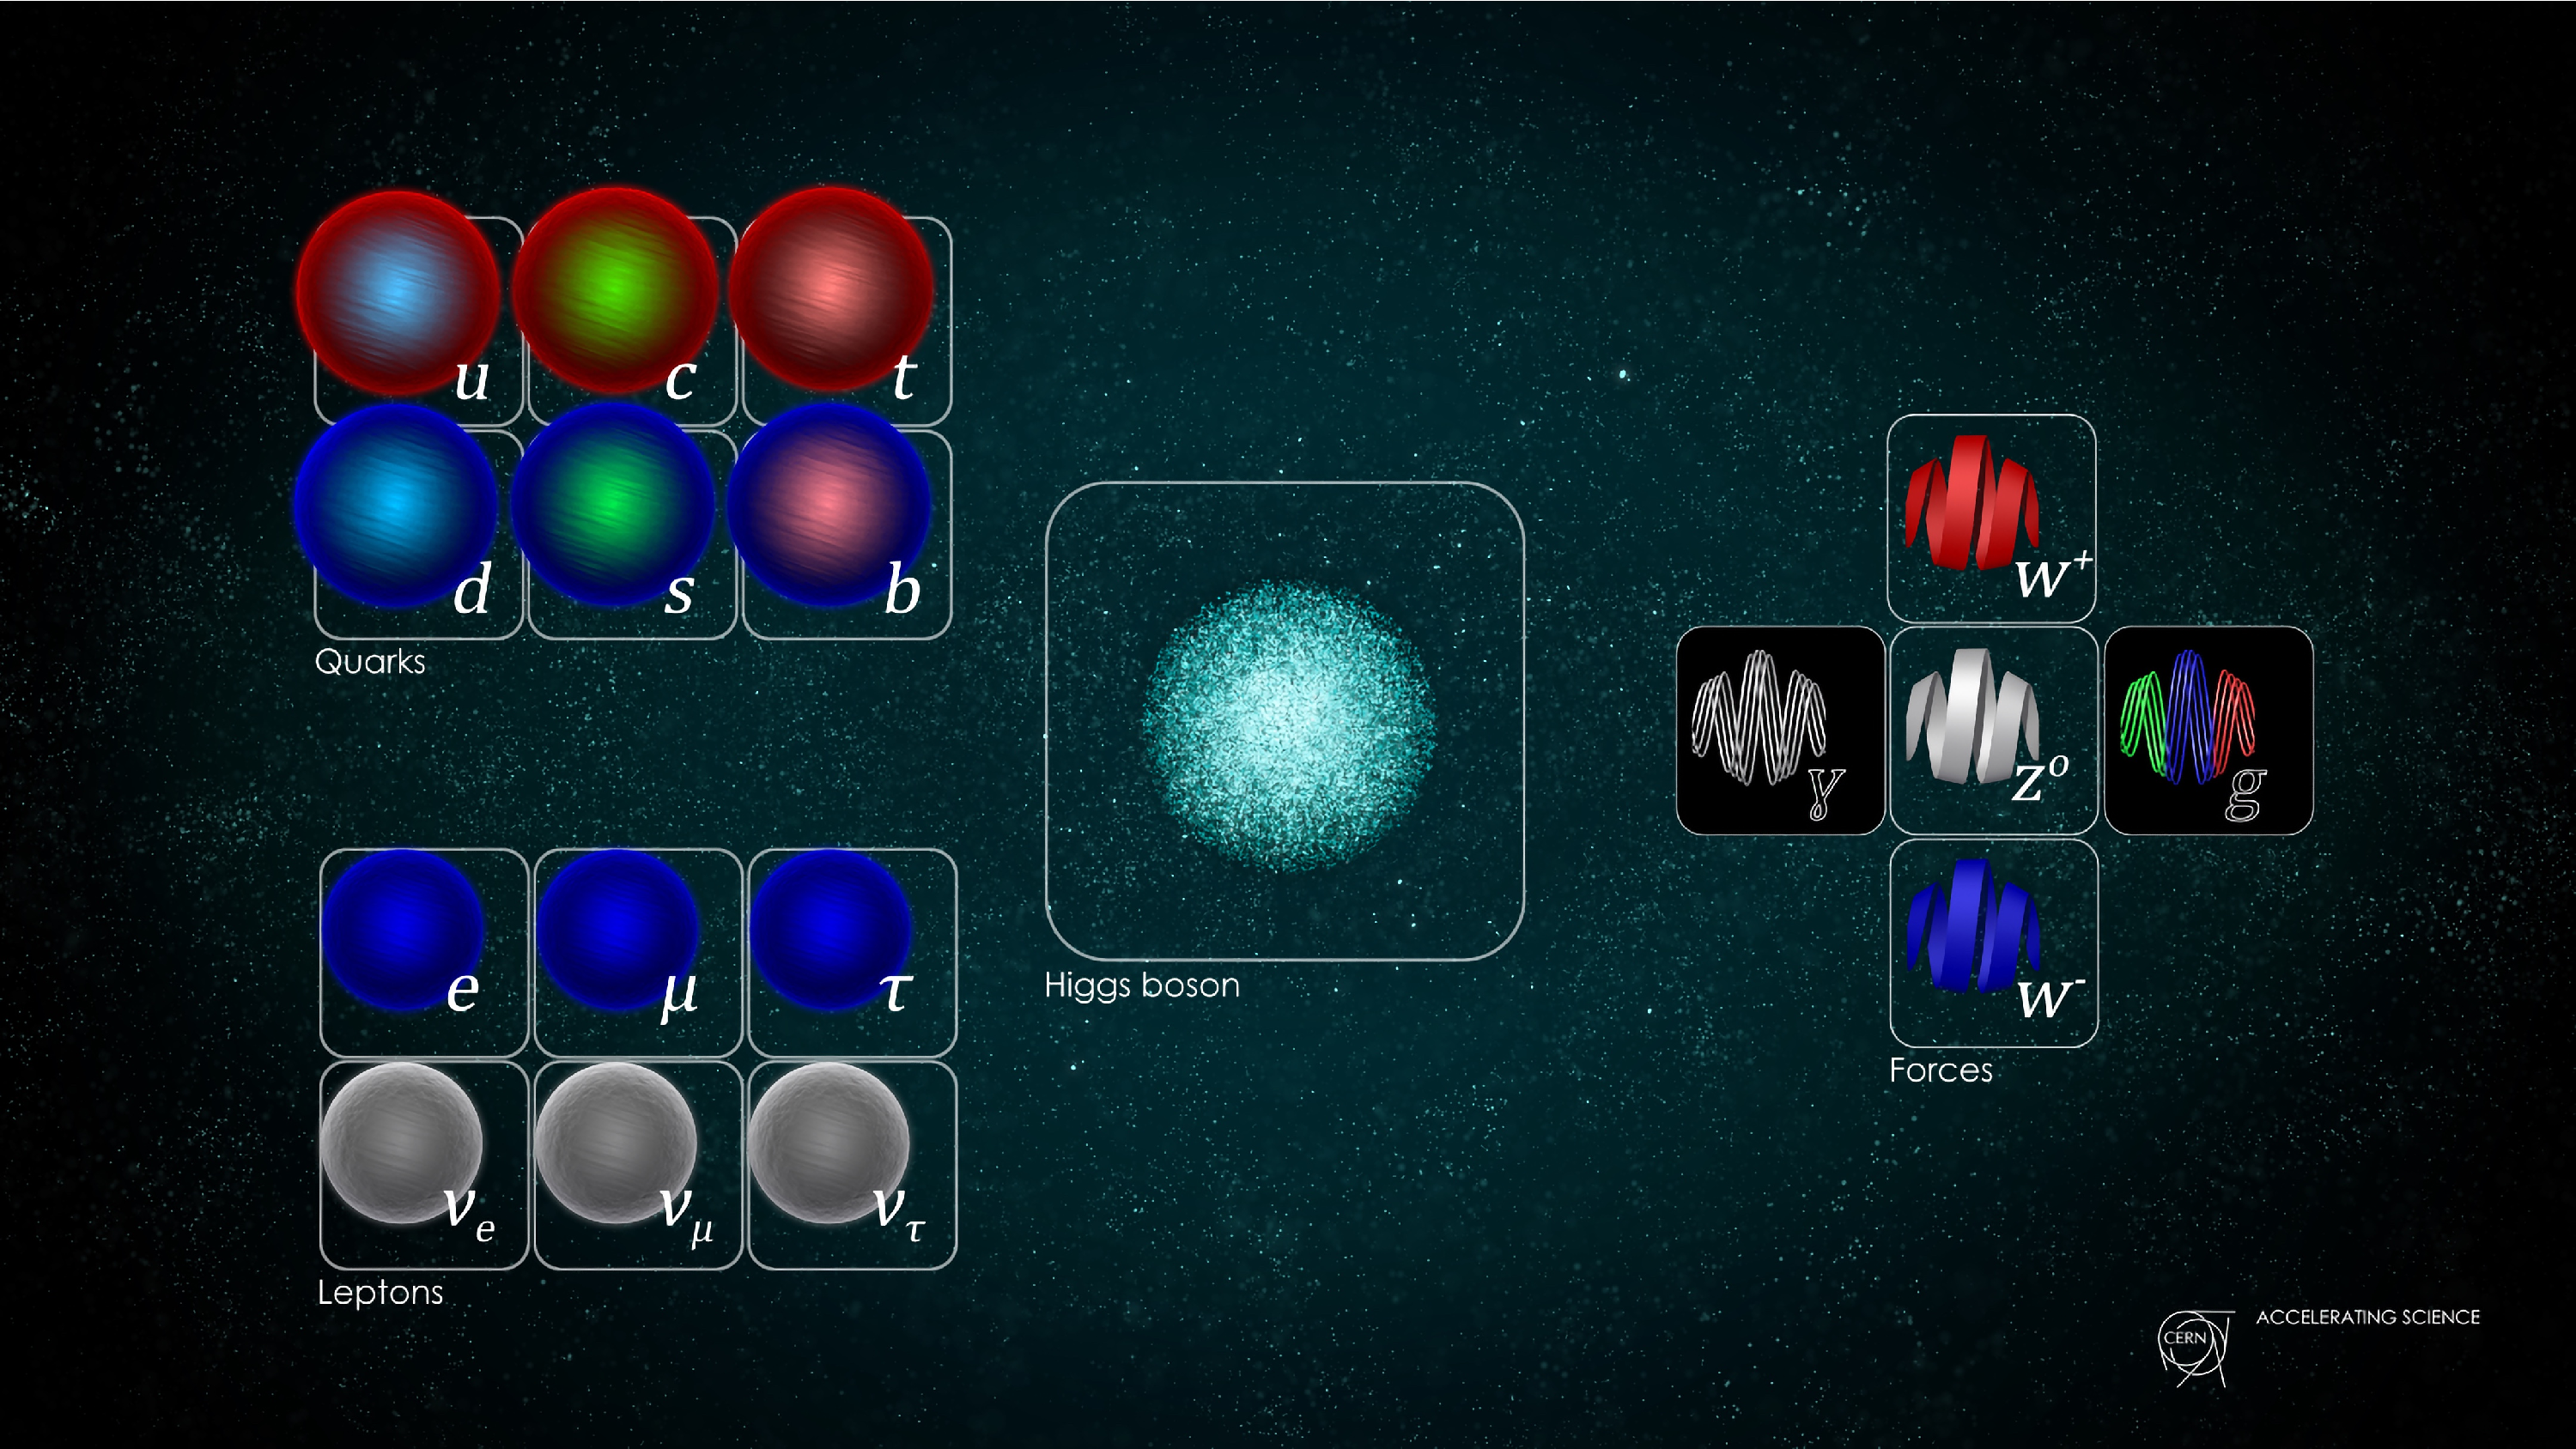
\includegraphics[width=0.9\linewidth]{files/StandardModel.pdf}
 	\caption{The Standard Model of Particle Physics\ \cite{cern_SM}.}\label{StandardModel}
\end{figure}

A first limitation of the Standard Model lies in its inability to provide a quantum description of gravity. A force-carrier of the gravitational force, the graviton, was hypothesized but not yet observed. The most accurate description of gravity remains the General Relativity, yet no framework currently exists that successfully unifies it with the Quantum Field Theory description of the Standard Model.
A second limitation arises from the fraction of the Universe that the Standard Model can account for. Indeed, only 5 $\%$ of the Universe, known as the baryionic matter, can be described, there is roughly 27 $\%$ of the Universe which is composed of so-called Dark Matter that the Standard Model is today unable to explain nor describe. The remaining 68 $\%$ of our Universe is made up by Dark Energy and is associated to the vacuum in space, yet its nature remains widely unknown too.\\

Aware of these limitations, physicist were first looking for outstanding phenomena that have been mostly ruled out by now. Significant efforts are being made towards precision measurement of the current theory in order to either further confirm the predictions or find inconsistencies hinting at unexplained phenomena and thus new Physics. For this reason, an upgrade of the current accelerator, the Large Hadron Collider (LHC), the High-Luminosity-LHC (HL-LHC) was proposed in order to obtain a fivefold increase of the instantaneous collision rate and a tenfold increase of the integrated luminosity with respect to the nominal LHC design values\ \cite{HL_LHC_report}.\\

Another limitation of the current LHC experiments like ATLAS or CMS is the geometrical acceptance their design can achieve. Indeed, the detectors are arranged in a cylindrical pattern centered around the LHC beam pipe, the detectors are hence very effective to detect heavy particles produced with large transverse momentum. On the contrary, if light particles were to be created in the very forward direction, they could be contained within the uncovered portion of space occupied by the beam pipe itself. Until proof of the contrary, some new Physics could also be hiding in these un-instrumented regions and some experiments already intend to use this incomplete acceptance to probe signals from weakly interacting and Long Lived Particles (LLPs) as suitable candidates for Dark Matter (DM).    
\clearpage 

\section{The FASER Detector: Looking Forward for New Physics}
The ForwArd Search ExpeRiment (FASER) is a detector located \SI{480}{\meter} downstream of the ATLAS Interaction Point (IP), benefiting from the curvature of the LHC to probe LLPs emitted in the very forward direction, initially contained within the uncovered acceptance of the experiment. 
The FASER detector was originally designed to detect charged decay of LLPs such as Dark Photons into an electron-positron pair. Although, in its current state, the detector is not able to distinguish between events in which one or more photons are produced. The FASER collaboration hence proposed in 2021 an upgrade of the original Preshower sub-detector with a high precision Tungsten-Silicon (W-Si) Preshower displaying its ability to resolve di-photons events from the decay of Axion-Like Particles (ALPs)\ \cite{PreShower_TP}. \\

The work presented in this thesis will first guide the reader through a description of the FASER detector and its original layout for the detection of charged decay products from LLPs. The reader will then be presented with the Physics program of FASER and why it was essential to unlock its potential for detection of neutral decay products such as di-photon signals. A theoretical description of an ALP model used for the proposal of the Preshower upgrade will then be given. The discussion will start with the motivation for ALPs, move to a phenomenological description of the specific ALP model simulated for this purpose and will finish with ALP production and decay within the FASER detector. 

\section{Development of Monolithic Silicon Pixel Detectors for HEP.}
\subsection{Motivation for a new detector technology}
The recent achievement in semiconductor technologies, and especially silicon-based devices, have paved the way for the development of the new detector technologies needed to overcome the challenges of future experiments. The important increase in number of collisions will be a real challenge for the experiment built within the specifications of the nominal LHC parameters. A complication that will need to be addressed is the increase in pile-up, the phenomenon in which the detector is not able to distinguish between tracks coming from different collisions of protons within the bunches. So far, particle tracking systems were relying only on the 3D information to deal with pile-up events, but the amount of such events will increase from roughly 50 up to 200 with the HL-LHC characteristics\ \cite{PhaseII_Atlas}.

The discriminating criteria to associate tracks to the correct collisions lies in the timing information associated to the reconstructed particle tracks, making these particle tracking systems 4D-trackers. The pile-up events are mostly contained within a time window of not more than \SI{200}{\pico\second}, slicing the beam crossing spot in consecutive exposures of \SI{30}{\pico\second}, the number of vertices per exposure would drop to current LHC pile-up levels\ \cite{PhaseII_CMS}. Some experiments like ATLAS\ \cite{PhaseII_Atlas} or CMS\ \cite{PhaseII_CMS} already foresee an upgrade of the detector layout including a timing layer in the pseudo-rapidity regions where the pile-up is the most important. \\

Traditionally, in order to obtain a time resolution of the order of tens of picoseconds, gas detectors such as the Multigap Resistive Plate Chambers (MRPCs) designed for the Alice Time Of Flight (TOF) detector\ \cite{MRPCs_AliceTOF}, have been a suitable solution. Although, the design and performance of such detectors is not compatible with the requirements of the 4D trackers. Indeed, as the trackers are located very close to the beam interaction point, they need good spatial resolution combined with a compact design but among all a capability to sustain high detection rates. Silicon based detectors offer many advantages in this regard which will later be discussed in \chref{ch:2}. \\

At the University of Geneva (UniGe), the development of monolithic silicon pixel detectors for timing applications has started in 2016 under the TT-PET project which proved that monolithic sensors can be used to reach time resolution of the order of \SI{110}{\pico\second} \cite{TTPET-110ps}. This already impressive performance was further improved over the years, now under the MONOLITH project, reaching in 2023 a time resolution of \SI{20}{\pico\second} for a sensor without internal gain layer. The sensor also demonstrated to remain fully efficient and offer time resolutions of the order of \SI{50}{\pico\second} even when operated at very low power densities of \SI{150}{\milli\watt/\centi\meter^2} \cite{Monolith_20ps}.

The breakthrough in performances can be associated to the implementation of Silicon Germanium Hetero Bipolar Transistors (SiGe HBTs) to produce very fast and low noise frontend electronics. The combination with monolithic implementation offers a sustainable solution, benefiting from the simplified assembly process and reduced production cost of monolithic designs in commercial Complementary Metal Oxide Semiconductor (CMOS) processes used in large-volume silicon foundries.

\subsection{Monolithic sensors for ultra-fast timing}
The MONOLITH project at UniGe aims at developing a new generation of monolithic silicon pixel detectors, improving the intrinsic time resolution limit of roughly \SI{30}{\pico\second} of current designs by an order of magnitude and providing at the same time high spatial resolution. 

The work presented in this thesis will first guide the reader through a description of semiconductors and how these can be used for particle detection. The formation of signal and its reading out will be presented alongside a comparison of hybrid and monolithic pixel detectors. This introductory part will be concluded by a discussion of the relevant factors to characterize radiation tolerance of this technology. 

Subsequently, the work performed for the characterization during testbeam campaigns at the SPS facility at CERN of two prototypes will be presented. The layout of the test set-up as well as the data taking methods will be introduced to further discuss the measurement of detection efficiency and timing resolution of these prototypes, notably under low power density operation.   

Finally, the radiation tolerance of the second prototypes discussed above will be discussed, again through some test at the SPS facility at CERN. The effect of different doses and the change in detection efficiency and timing resolution will be presented and discussed. 


\subsection{Monolithic sensors for TeV-scale photon detection }
The upgrade of the FASER Preshower detector can profit from the developments already achieved in monolithic silicon pixel detector technology to develop a high granularity silicon preshower detector. This design choice will reduce the overall cost and complexity of the upgrade that hybrid sensors would typically introduce. A dedicated front-end, still benefiting from the low noise performances of SiGe HBTs can be implemented to offer a sufficiently large dynamic range needed to resolve di-photons events in the detector. 

This part of the thesis will focus on the description of the FASER Preshower detector. The discussion will start by a description the requirements of the ASIC and how these influenced its design. The structure of the detector will be presented, along with the subdector components, the planes, and their subdivisions into modules, themselves composed of ASICs. The detector control and readout will also be presented to complete the description of the detector. 

The reader will then be presented with the diverse test performed in order to develop and assemble the FASER preshower detector. The discussion will start with the description and characterization of a pre-production ASIC, designed specifically to refine and test different design choices, leading to a description of the production ASIC. The qualification and commissioning of the detector will present the different assembly stages together with the characterization of ASICs and modules prior to installation. The development of the trigger and data acquisition software will be presented together with first results from testbeam campaigns demonstrating the functioning of the ASIC, its powering and its data acquisition system. 
